\chapter{Preparation and Ways to Access the  System}

\section {Installation on Raspberry Pi}
\index{Installation}
\index{RaZberry}

Before you can use the RaZberry solution, you need to complete your gateway hardware 
and install the software.

Here are two ways to install and start \zway:

\begin{itemize}
\item A:  You do not have Linux OS on your Raspberry Pi installed yet. Please download 
an SD card image (minimum 8 GB) from the download section of 
\murl{http://razberry.z-wave.me}. It is based on the Raspberry Pi distribution ``Jessie.’’

\item B (recommended): You already have a working Linux (Jessie) running. Log in and 
execute the following command line:

\begin{quote}
\cmdline{wget -q -O - http://razberry.z-wave.me/install | sudo bash}.
\end{quote}

\end{itemize}

You may need to configure the Wi-Fi access point of your Raspberry Pi in order to allow 
direct wireless access.

\section {Installation on other platforms using UZB}
\index{UZB}

\subsection {Unix-based Platforms}

Let’s assume you already have shell access to your system. You can download a binary 
distribution from \murl{https://razberry.z-wave.me/z-way-server}.

\begin{figure}
\begin{center}
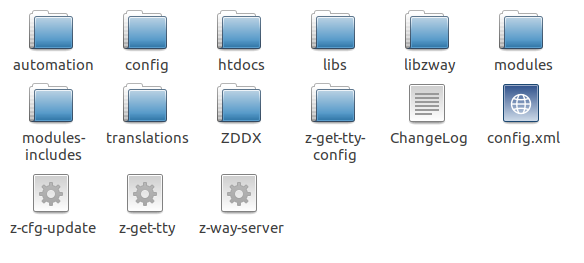
\includegraphics[width=0.7\textwidth]{pngs/cap3/rootfolder.png}
\caption{Folder Content of \zway}
\label{rootfile}
\end{center}
\end{figure}

and unpack it. The code can run on every place in the filesystem. Nevertheless, we 
recommend using \cmdline{/opt/z-way-server} as the folder to store the codebase. The 
folder content looks as shown in Figure \ref{rootfile}. For more information on the 
files and the file structure of \zway, please refer to Chapter \ref{clevelapi}.

\zway can then be started using the simple shell command from inside the \zway folder:

\begin{quote}
\cmdline{LD\_LIBRARY\_PATH=./libs ./z-way-server}
\end{quote}

Once the code is started, it is possible to access the standard user interface using 
\murl{http://localhost:8083}

To use Z-Wave, the correct port of the Z-Wave transceivers virtual serial port must be 
configured. Please  go to the user interface menu and open the app \app{Z-Way Network Access} 
as shown in Figure \ref{zwaynetworkapp}. for more information about \zway aps please refer 
to Chapter \ref{apps}.

\begin{figure}
\begin{center}
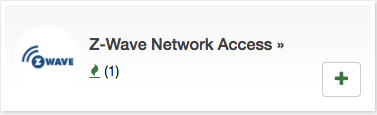
\includegraphics[width=0.4\textwidth]{pngs/cap3/zwavenetwork.png}
\caption{Z-Wave Network Access App}
\label{zwaynetworkapp}
\end{center}
\end{figure}

After checking the right virtual port created by the operating system, please configure 
this port name and save the settings. Now \zway should be up and running, and you may 
want to create a startup script to make sure \zway is running right after booting.

\subsection {Windows}
\index{Windows}

First, note that the Windows platform is only partly supported. There is a binary distribution 
for Windows, but it certainly lacks the level of testing required. Please use the binary 
Windows distribution at your own risk.

\begin{figure}
\begin{center}
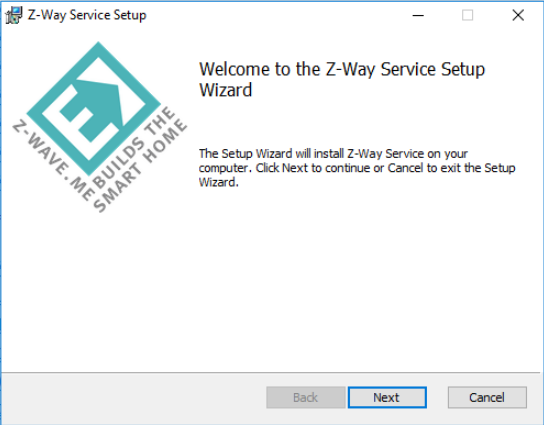
\includegraphics[width=0.6\textwidth]{pngs/cap3/winsetup1.png}
\caption{\zway Windows Setup Wizard}
\label{winsetup1}
\end{center}
\end{figure}

Install the MSI file and start it. You will see a nice wizard---see Figure \ref{winsetup1}
---guiding you through the setup process.


\begin{figure}
\begin{center}
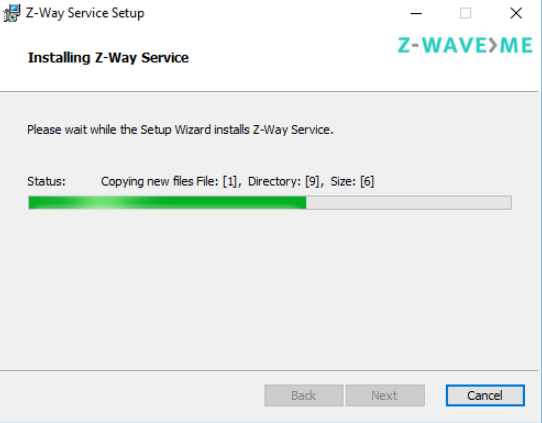
\includegraphics[width=0.6\textwidth]{pngs/cap3/winsetup2.png}
\caption{\zway Windows Installation}
\label{winsetup2}
\end{center}
\end{figure}

The files are installed on the folder of choice as shown in Figure \ref{winsetup2}.


\begin{figure}
\begin{center}
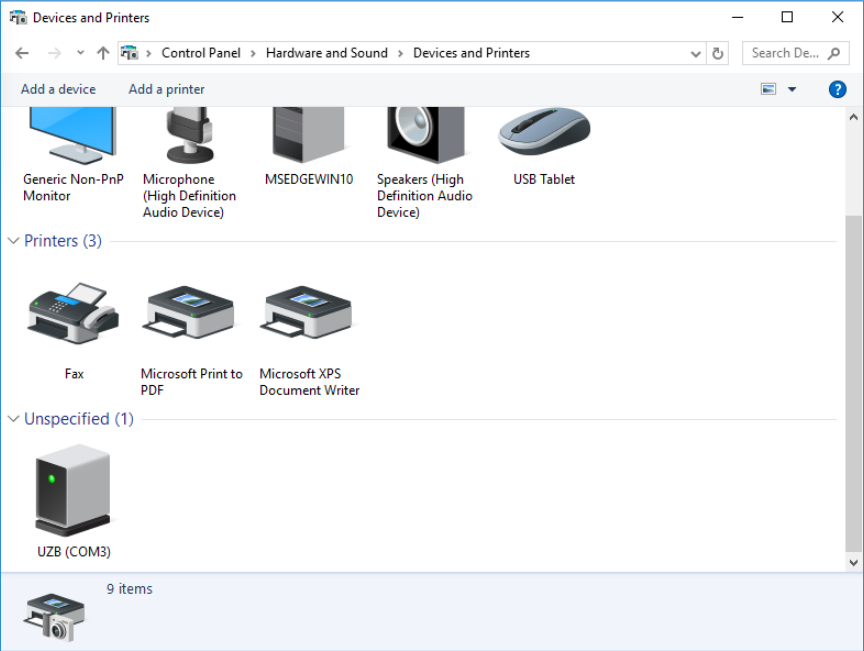
\includegraphics[width=0.6\textwidth]{pngs/cap3/winsetup3.png}
\caption{Windows Hardware manager with new COM port}
\label{winsetup3}
\end{center}
\end{figure}

If the UZB stick is plugged into the system, there is a new COM port created for this stick. 
Figure \ref{winsetup3} shows the Windows hardware manager with the new port. After passing 
the initial setup page, open the app \app{Z-Way Network Access} and double check the 
right COM port. Note that there is a very special syntax for the COM port 
\textbf{'\textbackslash \textbackslash.\textbackslash COM3'} for serial port 3.

Figure \ref{winsetup4} shows this dialog.

\begin{figure}
\begin{center}
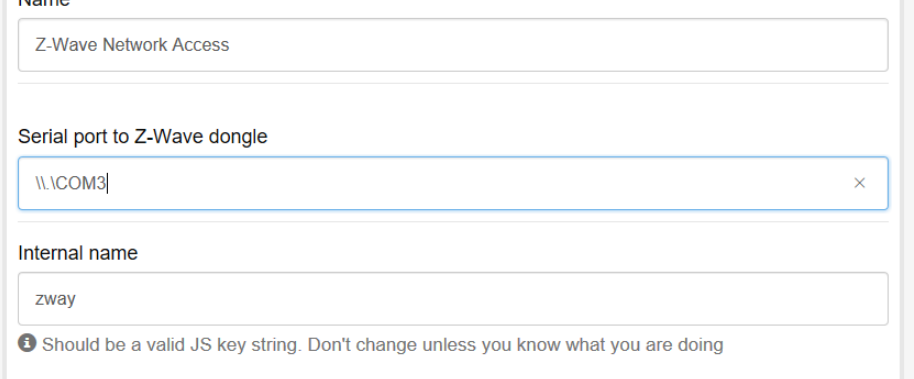
\includegraphics[width=0.6\textwidth]{pngs/cap3/winsetup4.png}
\caption{Z-Wave Network Access App with COM Port}
\label{winsetup4}
\end{center}
\end{figure}

Under Windows, \zway runs as a service. You find the service entry in the Windows Service 
Management as shown in Figure \ref{winsetup5}. This dialog also allows starting and stopping 
the service.

\begin{figure}
\begin{center}
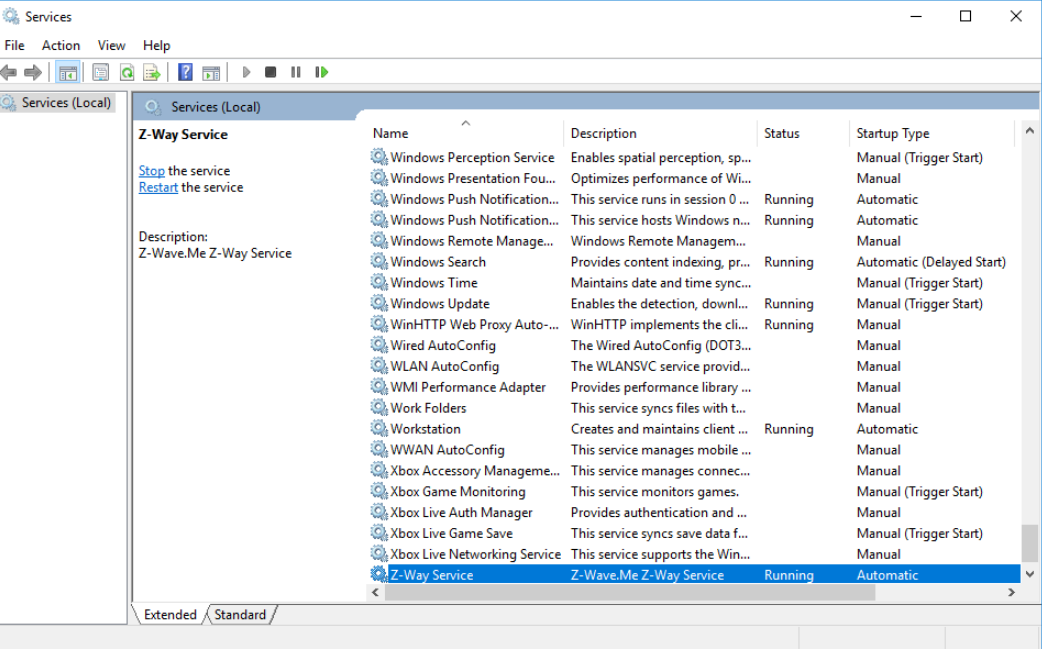
\includegraphics[width=0.8\textwidth]{pngs/cap3/winsetup5.png}
\caption{Z-Wave as Windows service}
\label{winsetup5}
\end{center}
\end{figure}

\section {Local and Remote Access}
\label{remoteaccess}
\index{Remote Access}

\zway can be accessed in several ways:

\begin{itemize}
\item Using a standard web browser\footnote{We recommend Chrome, Firefox, or Safari 
since we frequently see problems with MSIE.} on the controller’s IP address. There is an 
embedded webserver on Port 8083 providing the web pages of the user interface.
\item Using a standard web browser but the redirection service \murl{https://find.z-wave.me} The 
user interface is similar, but there is no need to be on the same IP network or to 
install an explicit port forwarding.
\item Use one of the native apps from Google Playstore or Apple iTunes. These will, 
however, use the two same services for local and remote access as mentioned above and 
will only render the user interface differently.
\item Use your own web or native app-based user interface. Again, you will then use one 
of the two options mentioned above.
\end{itemize}

Both the local access and the remote access using the find-service have their pros and 
cons as listed in Table \ref{compaccess}:

\begin{table}
\begin{tabular}{|p{0.15\textwidth}|p{0.35\textwidth}|p{0.35\textwidth}|}
\hline
Access &	Advantage & Disadvantage\\
\hline
Local IP Ethernet&	very fast, all data stays within own home & no secure connection due
to missing IP certificates, IP address must be known, no access from outside the home\\
\hline
Find Service &	worked independent of local network setting from everywhere, very safe
due to complete end-2-end security & depends on external service, more delays\\
\hline
Local IP WIFI&	very fast and secure & another WIFI access point, no access from outside the home  \\
\hline
\end{tabular}
\caption{Comparison of Access methods}
\label{compaccess}
\end{table}		

The initial access to the user interface must be done using one of the local access routes. 
Once \zway is running, the first access to the interface asks for some basic setup such 
as the admin password and an email address to recover this password. Figure \ref{init1} 
shows this screen.
The number provided in the title (1) is the unique \zwaydeviceid of the device and it will be needed 
in the future to access the controller remotely using the find service. 

\vspace{5mm}
\noindent\framebox{\noindent
\begin{minipage}{\dimexpr\linewidth-2\fboxrule-2\fboxsep\relax}
\begin{center}
{\fontsize{20}{28}\selectfont Please remember this \zwaydeviceid!}
\end{center}
\end{minipage}}
\vspace{5mm}


The  
\includegraphics[width=0.02\textwidth]{pngs/world.png} on the upper right side 
allows changing the interface language from 
standard English to your chosen language. If your language is not yet available, you 
may want to consider contributing a translation. Please refer to Chapter \ref{sec:translation} 
for details on how to do this.

\begin{figure}
\begin{center}
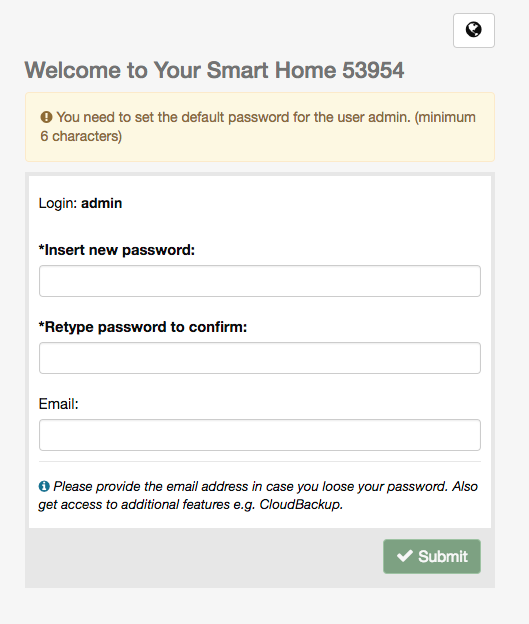
\includegraphics[width=0.5\textwidth]{pngs/cap3/init1.png}
\caption{Initial setup of the \zway User Interface}
\label{init1}
\end{center}
\end{figure}

The language selection can be used for the user interface from this time on, but it can 
be changed in \menu{
\includegraphics[width=0.02\textwidth]{pngs/smenu.png} > My Settings}.

Please note that the email address provided for email recovery will not be stored outside 
your controller, e.g. in a cloud service. This provides extra security but also means that 
certain processes like restore are a bit more complicated than is usual.

After completing the setup, a welcome screen will guide you through the system and 
introduce the basic user interface terms/dialogs.

\begin{itemize}
\item Element,
\item Element View,
\item Element Configuration,
\item Dashboard,
\item Event,
\item Timeline,
\item Apps
\end{itemize}

It also offers buttons for direct access to the two most common actions right after installation:

\begin{itemize}
\item Add a new physical device.
\item Add some virtual device, internet service or application.
\end{itemize}

After completing the setup, it is possible to access \zway using the find service, or install 
a native app for the mobile phone. Open the url \murl{https://find.z-wave.me/}

The dialog on this find service, as shown in Figure \ref{sh1}, is intentionally 
simple. It offers two ways to log in:

\begin{itemize}
\item Using your \zwaydeviceid, along with your login name (Example: '23333/admin') and 
your password for remote login and redirection
\item In case you use the service from a PC or a mobile phone within your home, the 
service will detect this and show the IP addresses of your \zway controllers. It 
is possible that a \zway controller has two IP interfaces (Ethernet + Wi-Fi). In 
this case, both addresses are shown. Clicking on the IP address will lead to the 
local IP login screen, as shown in Figure \ref{init2}, where only name (e.g. admin) and 
password are required.
\end{itemize}

\begin{figure}
\begin{center}
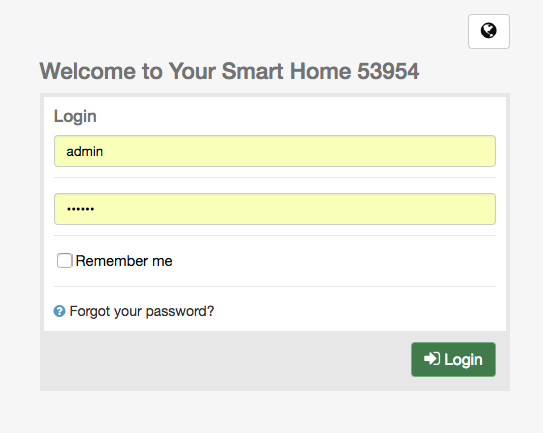
\includegraphics[width=0.5\textwidth]{pngs/cap3/init2.png}
\caption{Login on local IP address}
\label{init2}
\end{center}
\end{figure}

\begin{figure}
\begin{center}
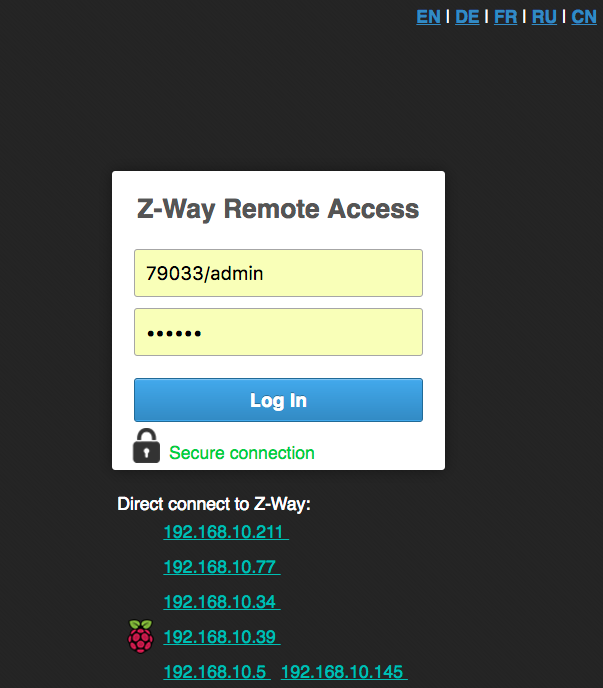
\includegraphics[width=0.5\textwidth]{pngs/cap3/sh1.png}
\caption{Remote Login Screen}
\label{sh1}
\end{center}
\end{figure}

The menu option \keystroke{Logout} in the setup menu of the user interface will terminate 
the session and return you to the login screen or the find service depending on how to 
log in. You can always force the termination of the find session by calling the 
URL \murl{https://find.z-wave.me/zboxweb}.

\section {Security and Privacy}
\index{Security}
\index{Privacy}

Security and privacy are of great importance. \zway tries to maximize security and privacy 
and will not compromise them in order to improve user experience and convenience.

\begin{itemize}
\item All user data including login name and email address are stored only locally, which 
means that the controller must be available and connected to restore passwords. We 
believe that this is a robust security and privacy measure.

\item \zway offers certain cloud-based services. This requires certain services and 
connections to the \zway cloud service:

\begin{itemize}
\item Right after boot-up, the \zway controller will connect to the find service 
announcing its presence. This is done using a reverse ssh service. The client side of this 
service is available on the \zway server and you can review its work and source code. 
If you don’t like this service, you can turn it off using the \zwshui. 
However, be prepared not to have the find service available anymore.

\item The backup to cloud service will also create a copy of your device data on the 
cloud service. This is very convenient and ensures that you have a backup file when 
needed. If you feel uncomfortable leaving a copy of your smart home configuration 
on the \zway cloud service, just don’t use this service and turn it off.

\end{itemize}

\item The find service allows https connection and provides a valid certificate issued by 
COMODO RSA Domain Validation Secure Server CA. Please check the validity of the 
certificate before using the find service. This means that the access using the find 
service has established a complete secure connection from the web browser via the 
find service to your controller at home.

\item There is no https access enabled to the local port. This is because there is no way 
to create a valid certificate on an IP address that is assigned dynamically using DHCP. 
It would still be possible to run encryption with https, but we believe that this would 
be mimicking security without having real security. That’s why we only keep http to 
send a clear message about the risk of accessing a local IP address. We strongly 
recommend doing an initial password setting and subsequent local access using Wi-Fi 
only since Wi-Fi comes with its own very secure encryption based on WPA.

\end{itemize}

